\section*{Visualização do Sistema}

Nesta fase do processo de Concepção, o seu objetivo é entender completamente qual a intenção ou objetivo do cliente: para quê ele quer um sistema? Como ele deve funcionar? Quem vai usar? Qual problema ele resolve? Tudo isso deve ser levantado nesse segundo momento, geralmente uma reunião presencial ou virtual. É um evento que marca que, realmente, o projeto vai ser desenvolvido! Porém, como ainda se trata de um processo inicial, não dá pra dizer que o que for dito aqui será uma verdade absoluta até o final do projeto. Na verdade, isso será definido na próxima fase, que é o processo de Elaboração.

A abordagem mais recomendada nesse tipo de conversa, para visualizar o sistema, é utilizar um esquema de mapa mental. Isso porque ele é simples, de fácil entendimento entre as duas partes: desenvolvedor e interessado. Ele funciona como uma união, uma ponte de comunicação entre o que o cliente quer e o que você vai precisar desenvolver.

Tente construir um modelo como este:

\begin{figure}[H]
	\centering
	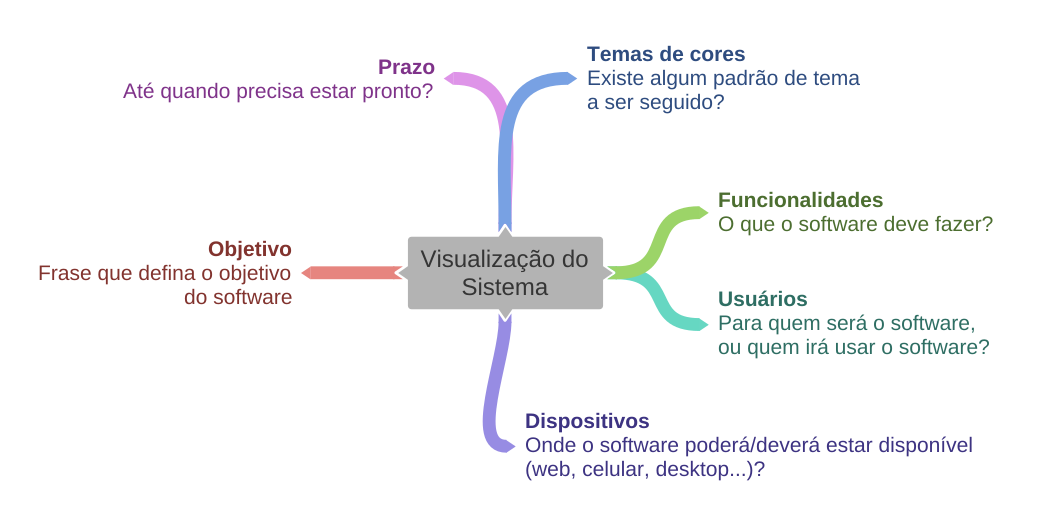
\includegraphics[width=\textwidth]{Visualizao_do_Sistema.png}
\end{figure}

Explicando, desenhe um mapa cujo centro pode ser o nome do sistema, se já existir, ou um nome que o caracterize. Deste centro, devem sair seis ramificações seguindo a seguinte ordem:

\begin{itemize}
    \item \textbf{Objetivo:} constituído por uma frase curta, sucinta e objetiva que consiga descrever para quê vai servir esse sistema. Não precisa pensar ou elaborar muito, algo com as suas palavras ou as do cliente. Essa definição ajuda a responder as próximas questões;
    \item \textbf{Usuários:} quais são as pessoas, os atores, que vão usar esse sistema? Dessa ramificação devem sair os nomes de quem vai ter acesso ou quem vai efetivamente usar a aplicação;
    \item \textbf{Funcionalidades:} o que os usuários vão fazer? Quais ações eles terão disponíveis? As funcionalidades estão bastante ligadas aos usuários. Sua definição nesse momento também pode ser bastante rápida e enxuta, apenas para entender a serventia do sistema, alinhada ao objetivo já definido;
    \item \textbf{Dispositivos:} por onde os usuários vão acessar o sistema? Essa questão é importante para entender qual será a arquitetura do sistema, ou seja, qual tipo de tecnologia você vai precisar empregar no desenvolvimento da solução;
    \item \textbf{Prazo:} não precisa ser uma data bem definida, aqui é interessante ter noção do que o seu cliente espera, qual a expectativa dele. Esse também é um ponto importante de negociação, para se discutir desde o começo, evitando problemas futuros;
    \item \textbf{Temas de cores:} verifique se já existe alguma regra estilística que você deverá respeitar, se essa responsabilidade será de outra pessoa ou se fica de livre escolha sua.
\end{itemize}


Esse modelo de mapa pode e deve ser usado durante a conversa mesmo! Para desenhá-lo, a depender das circunstâncias, você pode usar caneta e papel, ou se possível, ferramentas de desenho digitais.

**Dica de ferramenta**
Para desenhar mapas mentais, eu gosto e utilizo o [Coggle](https://coggle.it/). É uma ferramenta gratuita e de fácil utilização para construção de mapas rápidos e bonitos.

**Exemplo de utilização**
[Neste vídeo](https://youtu.be/brfNJdwhlDA), eu explico como realizar esta etapa de Visualização do Sistema de maneira prática, simulando o levantamento de um aplicativo para alunos universitários.

Se durante a conversa você achar necessário, algo que pode ajudar é fazer um fluxo de operação, quando aplicável. O Fluxo de Operação é um desenho de telas, que mostra o caminhamento dentro do sistema e já ilustra e inclui algumas das funcionalidades. Por exemplo, algo mais ou menos assim:

\begin{figure}[H]
	\centering
	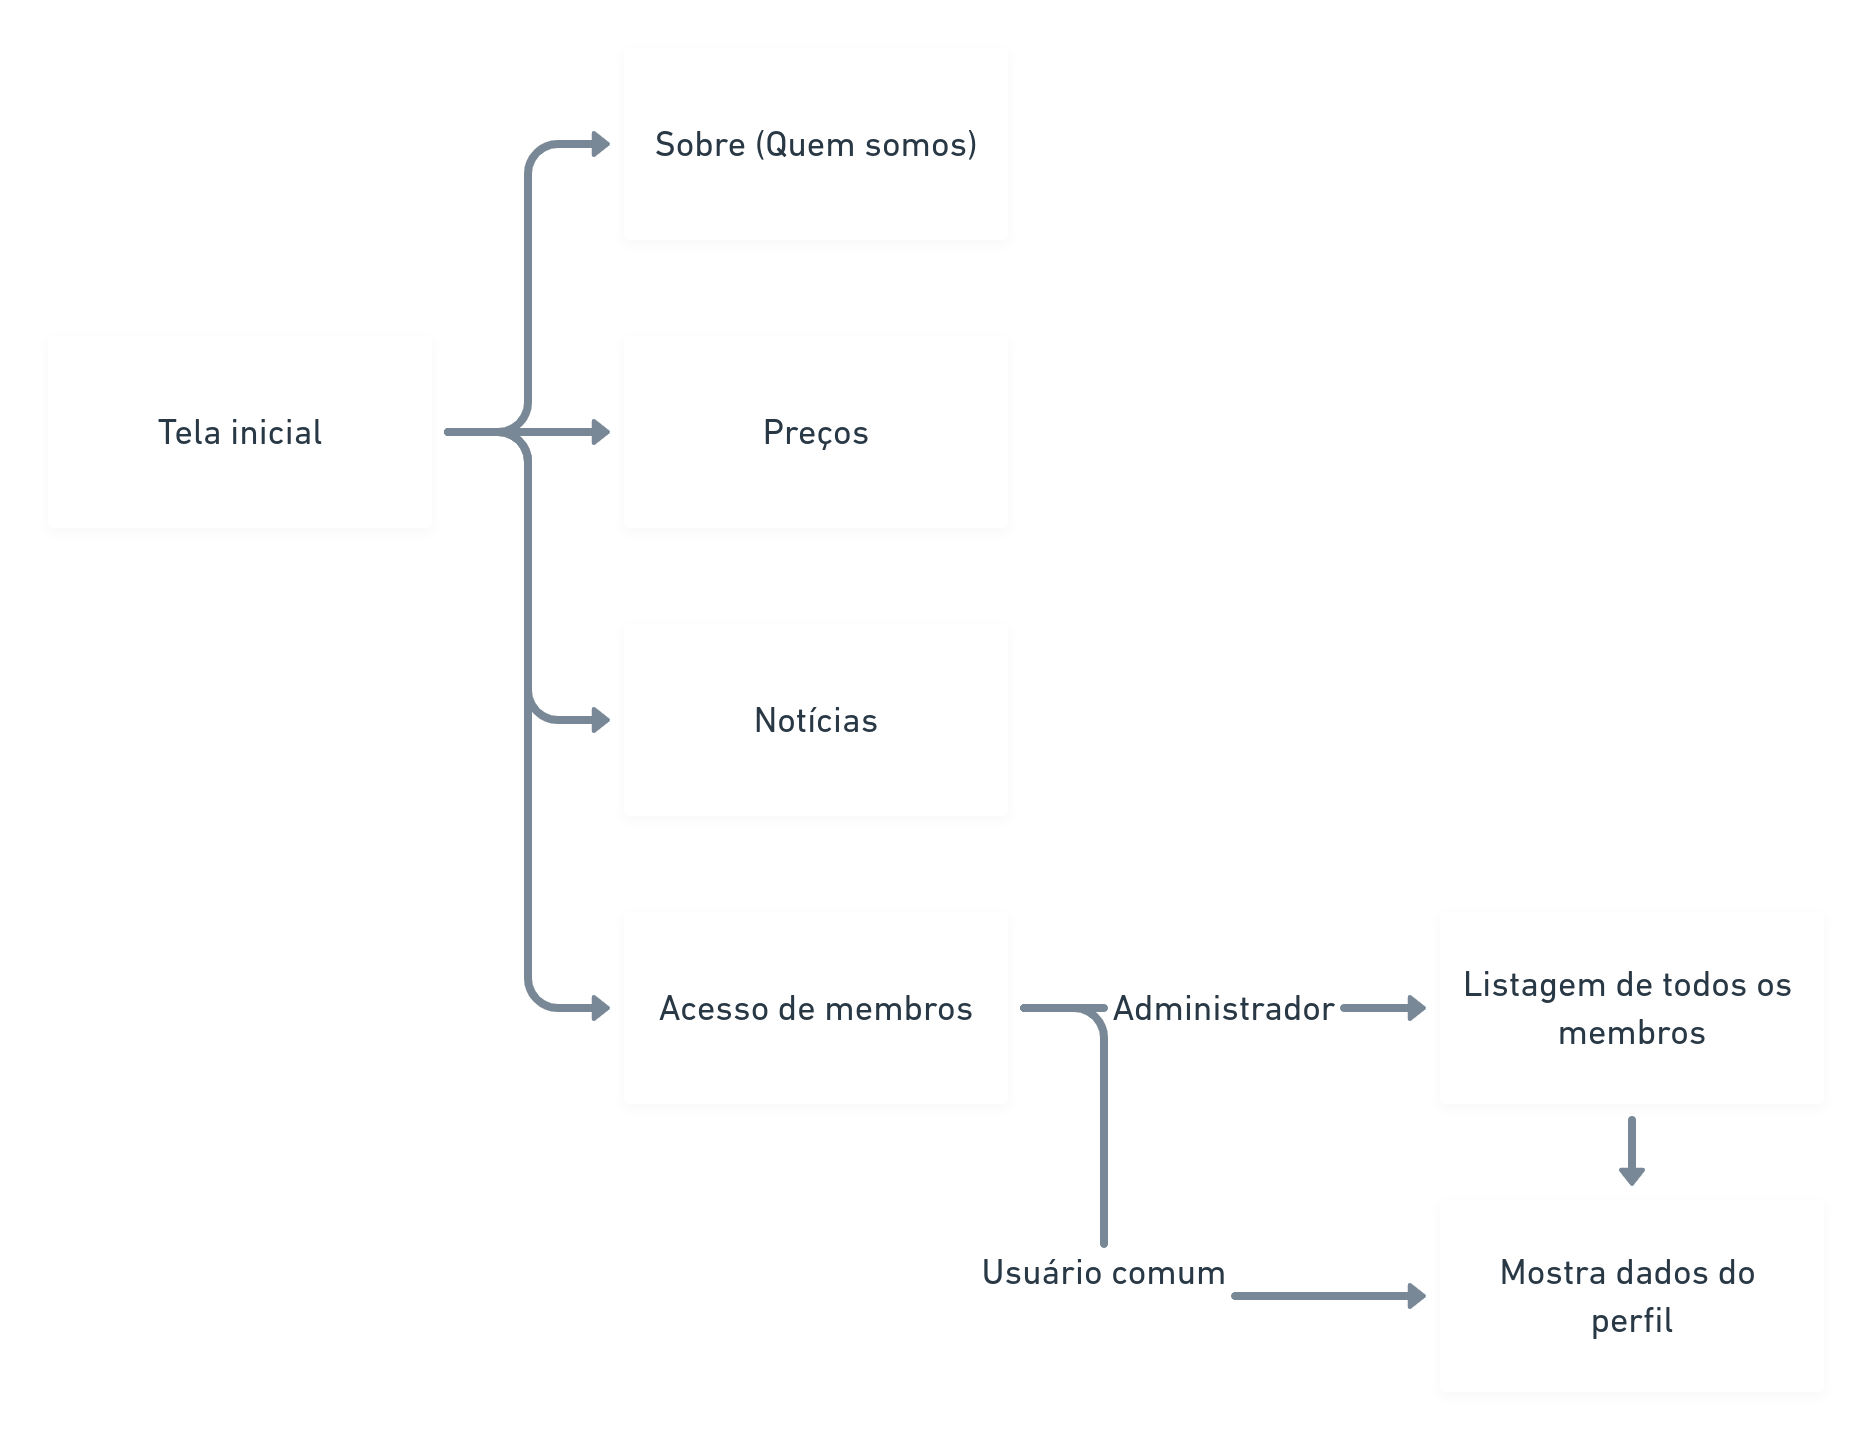
\includegraphics[width=\textwidth]{Postagens2x.png}
\end{figure}

Esse fluxo pode representar a estrutura de um site simples, como um exemplo didático do que o Fluxo de Operação quer dizer.

**Dica de ferramenta**
Esse tipo de desenho fica legal quando se usa o [Whimsical](https://whimsical.com/). Similar em facilidade ao Coggle, mais voltado para esse tipo de desenho de fluxogramas e semelhantes.

Geralmente, com a conversa e com o mapa mental feito, você já tem material suficiente para seguir para a próxima fase. Interessante que a construção desse mapa também ajuda a levantar várias questões e dúvidas, e já responde muitas também. A carga de informação e esclarecimento é bastante alta.

Na próxima fase, começa a Elaboração do sistema. É um processo mais formal, que parte de você para o cliente, onde você vai mostrar e detalhar como o sistema vai funcionar, o que vai ser preciso pra isso, quanto tempo vai levar e quanto vai custar.

**Quanto tempo leva?**
A fase de concepção geralmente é bastante rápida. Pode acontecer tudo no mesmo dia. É recomendado que essa fase dure no mínimo dois dias, e no máximo duas semanas.